\documentclass[11pt]{article}

\usepackage[utf8]{inputenc}

\usepackage{amsmath, bm}
\usepackage{graphicx}
\usepackage{amssymb}
\usepackage{float}
\usepackage{caption}
\usepackage{subcaption}
\usepackage{hyperref}
\usepackage{tikz}
\usepackage{layout}
\usepackage{wrapfig}

\usepackage[margin=1in]{geometry}
\usepackage{listings}
\usepackage{xcolor}
\usepackage{color, colortbl}
\usepackage{textgreek}
\usepackage{mathrsfs}
\usepackage{savetrees}

% 12 pt font
\renewcommand{\normalsize}{\fontsize{12pt}{\baselineskip}\selectfont}

\begin{document}

\title{4A7 Transonic Wing Design}
\author{lwp26}
\date{May 2024}
\maketitle

\section{Introduction}


The development of high-efficiency aerofoils, can significantly improve the overall performance of an aircraft.
The Breguet range equation, which calculates the range of an aircraft, directly depends on the flight speed and lift to drag ratio of the wing:

\begin{equation}
S = \frac{U}{g}\frac{L/D}{\text{sfc}} \log \left( \frac{W_\text{start}}{W_\text{end}} \right)
\end{equation}

where $S$ is the range, $U$ is the flight velocity, $g$ is the acceleration due to gravity, $\text{sfc}$ is the specific fuel consumption of the engine, and $W_\text{start}$ and $W_\text{end}$ are the initial and final weights of the aircraft, respectively.
This shows increasing flight speed and lift to drag ratio will increase the range of the aircraft.

\section{Maximum Lift, Minimum Drag}

Previous work in subsonic airfoil design showed the importance of the boundary layer growth on the viscous drag of the wing.
Adjustments were made to surface curvature, changing pressure gradients in effort to delay transition and separation, minimising boundary layer growth \cite{SA1_report}.

The difficulty with transonic airfoil design is that there is an additional source of drag, known as wave drag, which is caused by the formation of shock waves on the wing surface.

% the curvature of the top surface was increased and decreased in certain places
% a high amount of curvature at the leading edge provides rapid expansion to the suction peak, maximising lift here.
% the first spline point had to be negative to ensure no spline inflection point

% a very small amount of curvature is maintained around the top surface to prevent further expansion in the supersonic region,
% and to allow the reflected expansion lines to compress the flow, reducing the shock strength.
% more flat and concave curvatures were tested increased end curvature, increasing back pressure and caused a two shocks to form

% after the region of small curvature, just behind where the shock is located at operating conditions, there is high curvature to return to the surface back to the trailing edge.

% at the end of the upper surface, there is some concave geometry which produces downforce. 
% this is bad for lift, 

The designed airfoil cross-section is shown in Figure \ref{fig:airfoil}.


% reference SA1 wing analysis report

\begin{figure}[H]
    \centering
    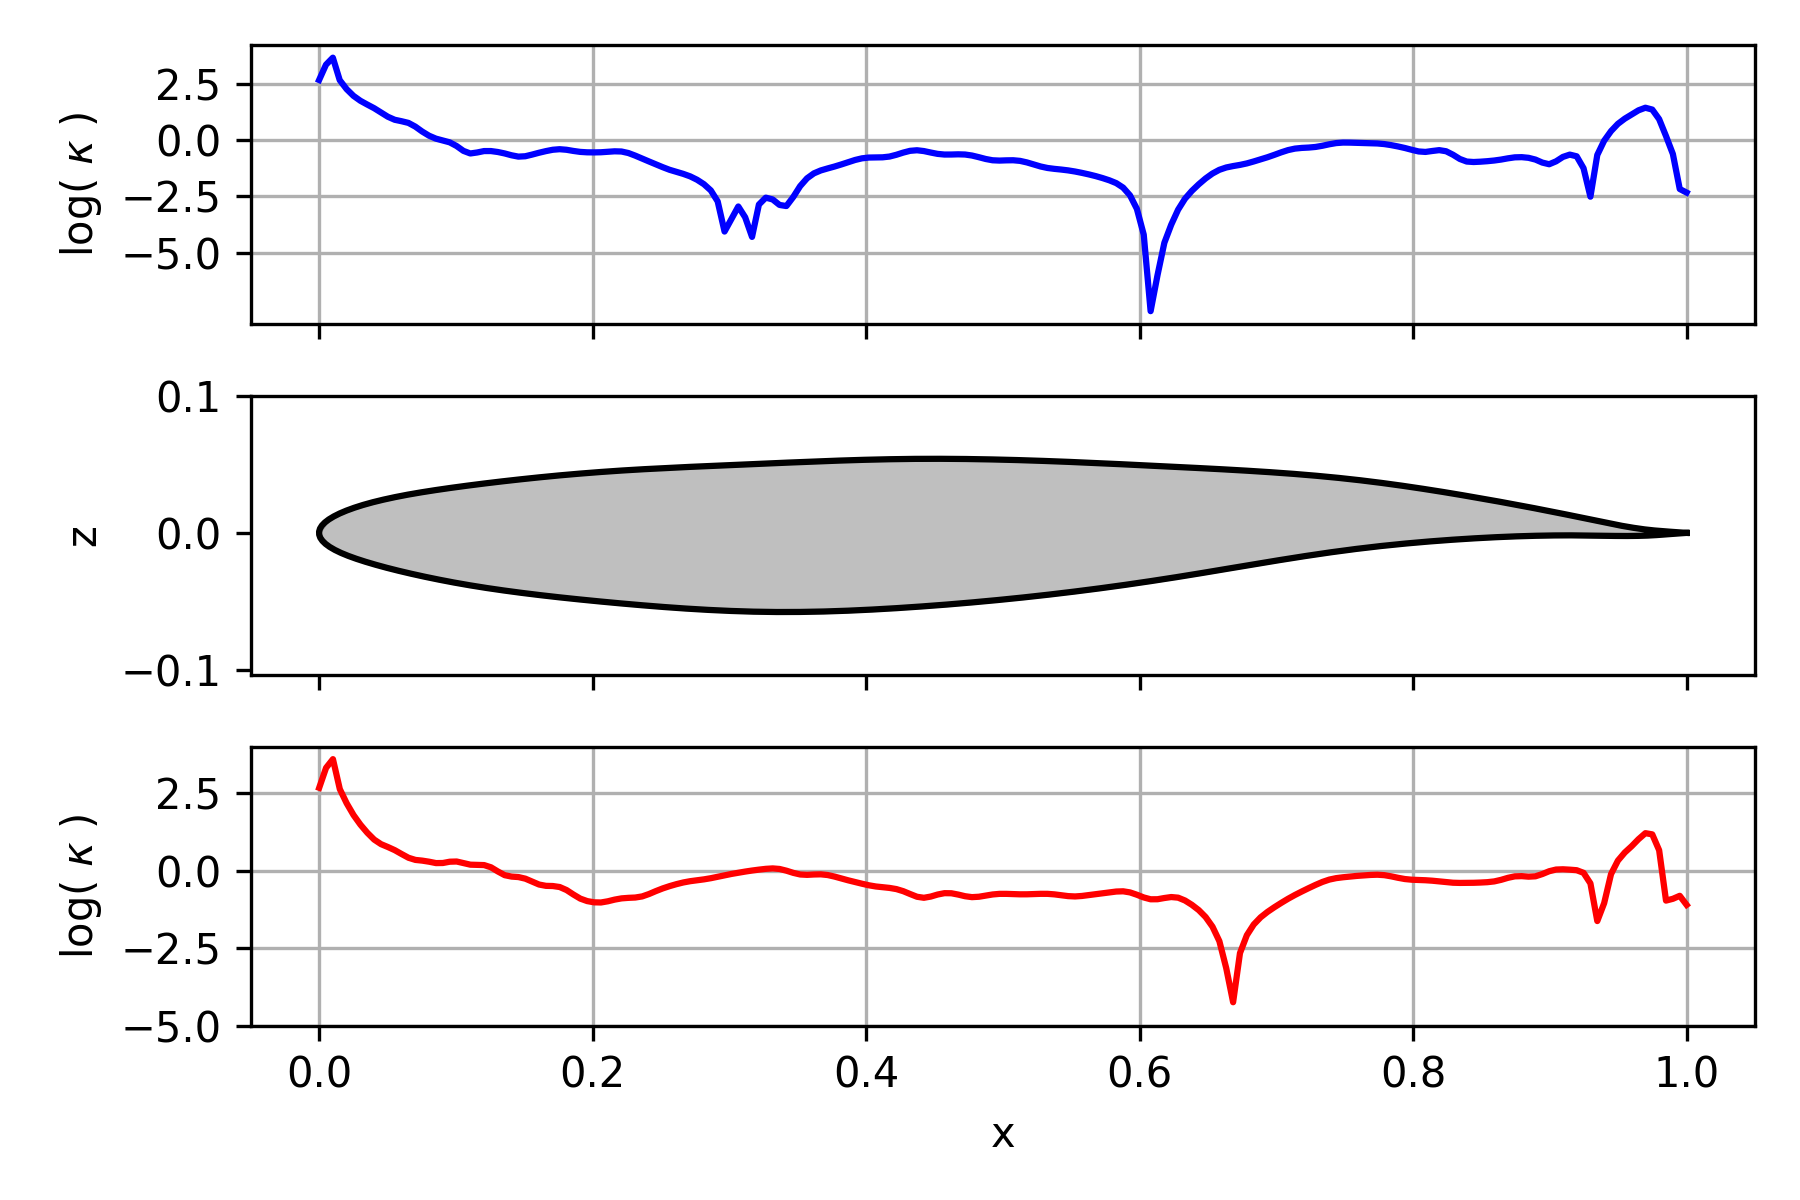
\includegraphics[width=0.6\textwidth]{figures/airfoil.png}
    \caption{Aerofoil cross-section}
    \label{fig:airfoil}
\end{figure}


\begin{figure}
    \centering
    \begin{subfigure}[t]{0.45\textwidth}
        \centering
        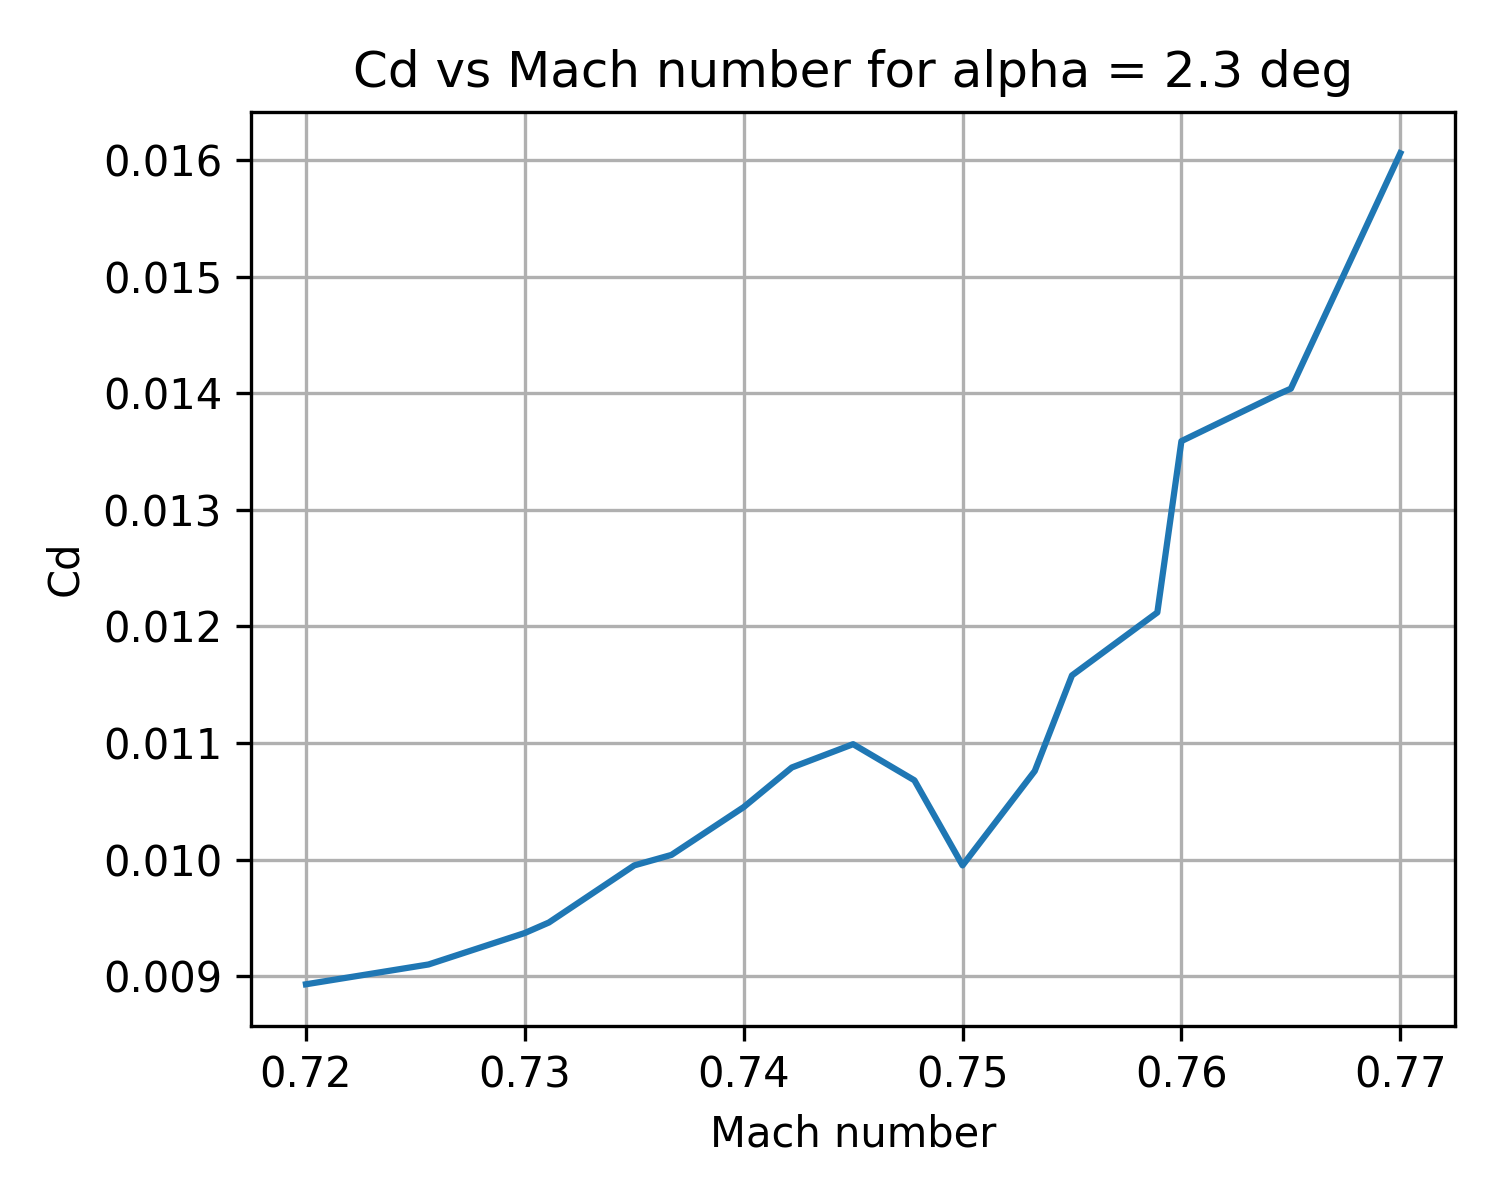
\includegraphics[width=\textwidth]{figures/cd_vs_mach.png}
        \caption{Drag coefficient vs Mach number}
        \label{fig:pressure_distribution}
    \end{subfigure}
    \begin{subfigure}[t]{0.54\textwidth}
        \centering
        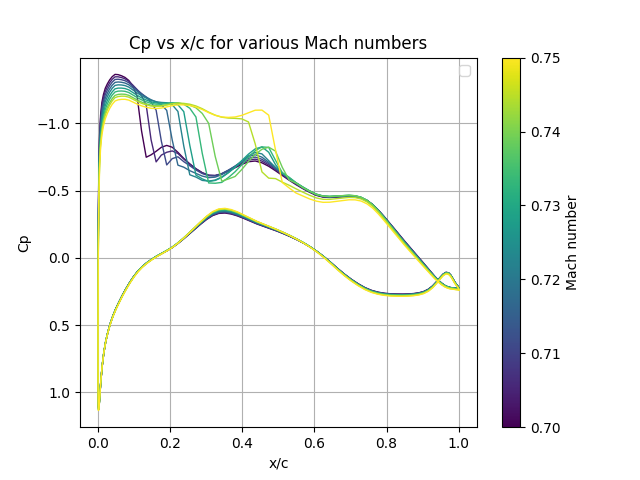
\includegraphics[width=\textwidth]{figures/cp_vs_xc_machs.png}
        \caption{Pressure coefficient distribution for different Mach numbers}
        \label{fig:mach_distribution}
    \end{subfigure}
\end{figure}


\section{Buffet Line}

Buffet is complex unstable interaction between the shockwaves and boundary layers and can produce large amplitude pressure fluctuations on the wing surface.
This can be damaging to the aircraft structure and cause a loss of control [?].

There are various measures to detect the onset of buffet
\begin{itemize}
    \item Shock entry Mach number
    \item Trailing edge shape factor
    \item High Mach numbers close to trailing edge
    \item Trailing edge pressure coefficient rise
\end{itemize}
These are quantified in the non-dimensional buffet factors, seen on Figure \ref{fig:buffet_classification}.

\begin{figure}[H]
    \centering
    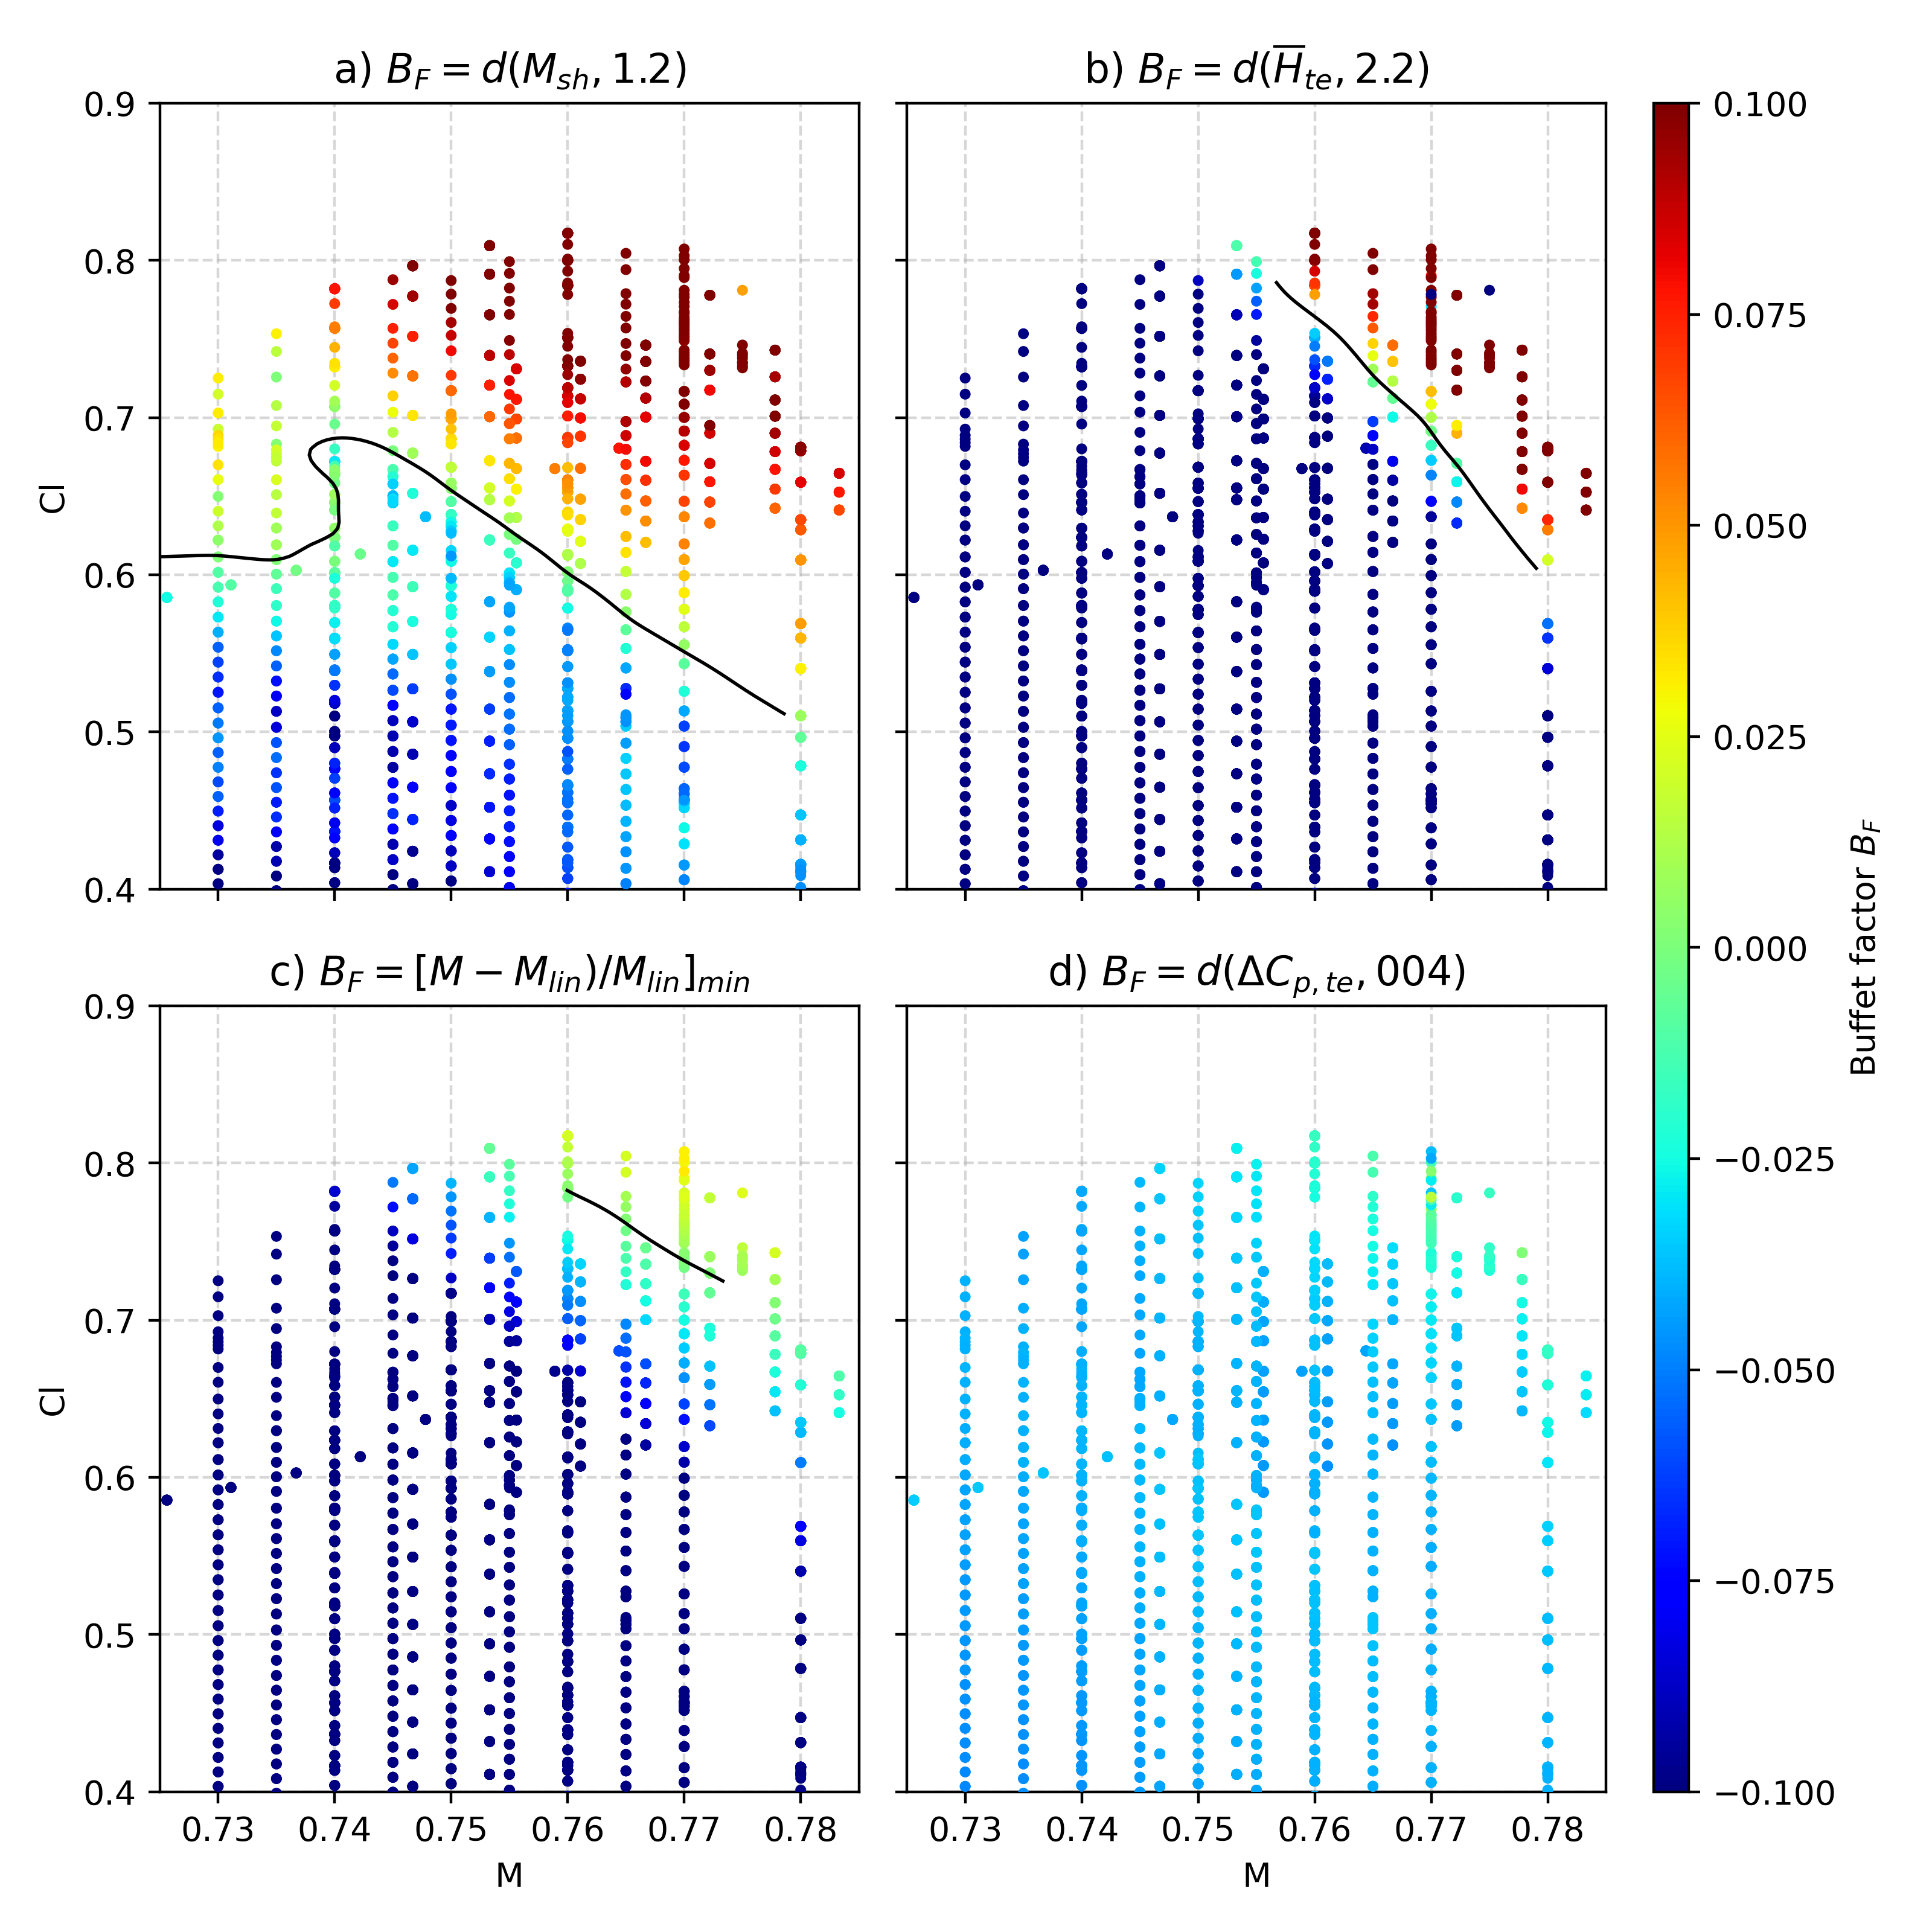
\includegraphics[width=0.8\textwidth]{figures/buffet_classification.png}
    \caption{Buffet factors at a range of Mach numbers and lift coefficients}
    \label{fig:buffet_classification}
\end{figure}

\begin{thebibliography}{9}

    %Endres, SC, Sandrock, C, Focke, WW (2018) “A simplicial homology algorithm for lipschitz optimisation”, Journal of Global Optimization.

      \bibitem{SA1_report}
      L. W. Pender
      \emph{SA1 Wing Analysis Final Report}
      University of Cambridge,
      2024.
    
      \bibitem{handout}
      J. Jarret
      \emph{4A7 Transonic Wing Design Handout}
      University of Cambridge,
      2024.
    
\end{thebibliography}

\end{document}